\documentclass{standalone}
\usepackage{tikz}
\usetikzlibrary{patterns, positioning}


\begin{document}
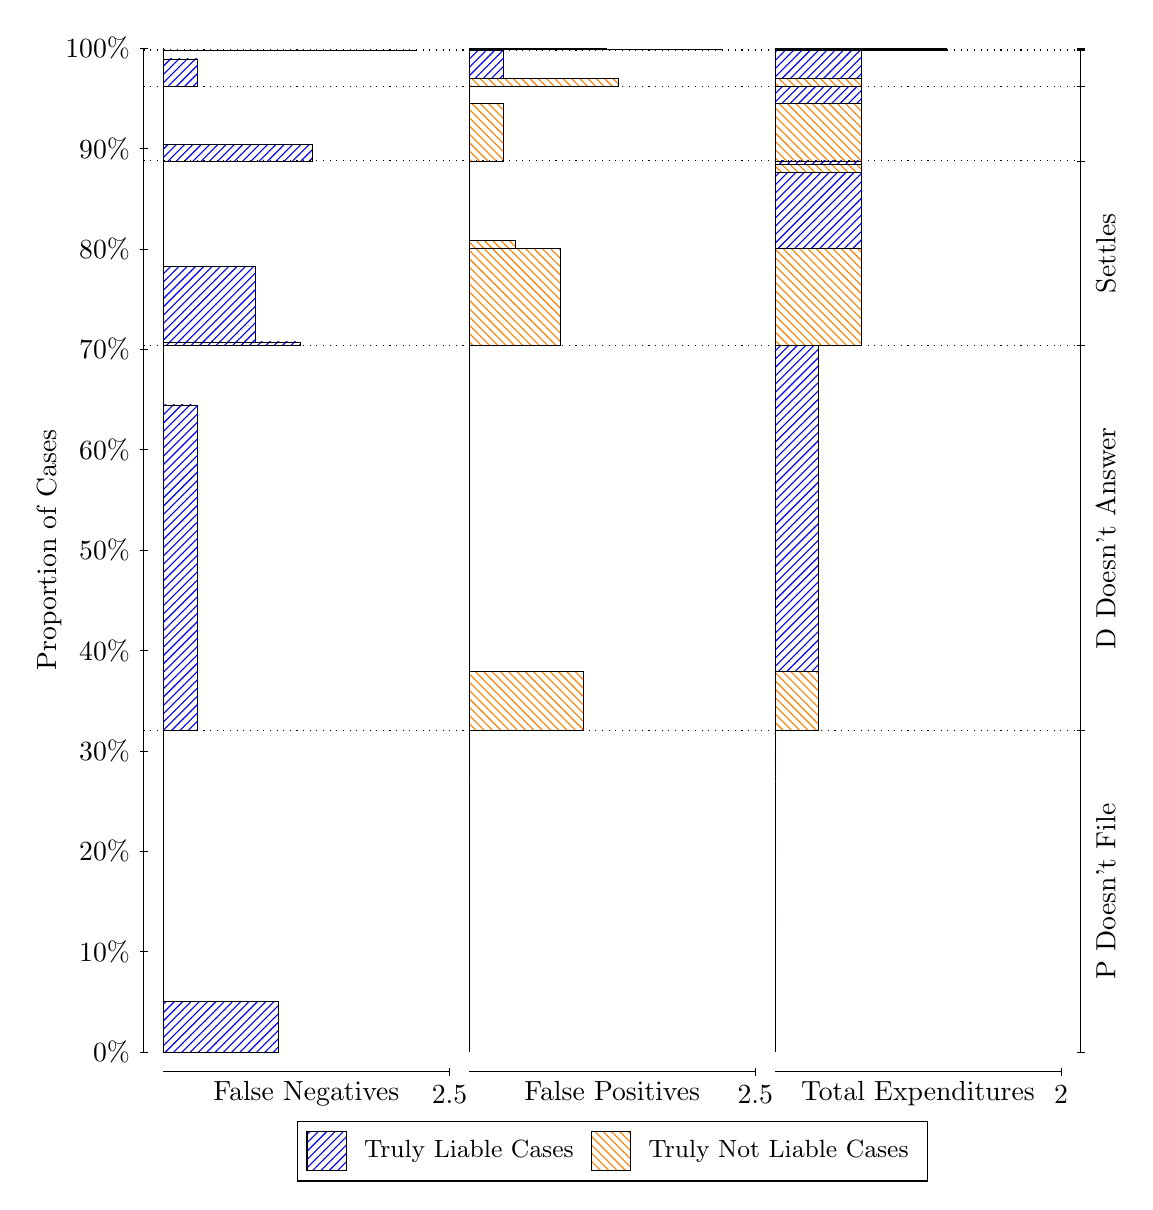
\begin{tikzpicture}
\draw[black, very thin] (1.5,1.75) -- (1.5,14.5);
\node[rotate=90, text=black, anchor=center] at (0.3, 8.125) {Proportion of Cases};
\draw[black, very thin] (1.45,1.75) -- (1.55,1.75);
\node[text=black, anchor=east] at (1.45, 1.75) {0\%};
\draw[black, very thin] (1.45,3.025) -- (1.55,3.025);
\node[text=black, anchor=east] at (1.45, 3.025) {10\%};
\draw[black, very thin] (1.45,4.3) -- (1.55,4.3);
\node[text=black, anchor=east] at (1.45, 4.3) {20\%};
\draw[black, very thin] (1.45,5.575) -- (1.55,5.575);
\node[text=black, anchor=east] at (1.45, 5.575) {30\%};
\draw[black, very thin] (1.45,6.85) -- (1.55,6.85);
\node[text=black, anchor=east] at (1.45, 6.85) {40\%};
\draw[black, very thin] (1.45,8.125) -- (1.55,8.125);
\node[text=black, anchor=east] at (1.45, 8.125) {50\%};
\draw[black, very thin] (1.45,9.4) -- (1.55,9.4);
\node[text=black, anchor=east] at (1.45, 9.4) {60\%};
\draw[black, very thin] (1.45,10.675) -- (1.55,10.675);
\node[text=black, anchor=east] at (1.45, 10.675) {70\%};
\draw[black, very thin] (1.45,11.95) -- (1.55,11.95);
\node[text=black, anchor=east] at (1.45, 11.95) {80\%};
\draw[black, very thin] (1.45,13.225) -- (1.55,13.225);
\node[text=black, anchor=east] at (1.45, 13.225) {90\%};
\draw[black, very thin] (1.45,14.5) -- (1.55,14.5);
\node[text=black, anchor=east] at (1.45, 14.5) {100\%};

\draw[black, very thin] (13.4,1.75) -- (13.4,14.5);
\draw[black, very thin] (13.35,1.75) -- (13.45,1.75);
\node[anchor=west] at (13.35, 1.75) {};
\draw[black, very thin] (13.35,5.8296) -- (13.45,5.8296);
\node[anchor=west] at (13.35, 5.8296) {};
\draw[black, very thin] (13.35,10.719) -- (13.45,10.719);
\node[anchor=west] at (13.35, 10.719) {};
\draw[black, very thin] (13.35,13.066) -- (13.45,13.066);
\node[anchor=west] at (13.35, 13.066) {};
\draw[black, very thin] (13.35,14.008) -- (13.45,14.008);
\node[anchor=west] at (13.35, 14.008) {};
\draw[black, very thin] (13.35,14.468) -- (13.45,14.468);
\node[anchor=west] at (13.35, 14.468) {};
\draw[black, very thin] (13.35,14.481) -- (13.45,14.481);
\node[anchor=west] at (13.35, 14.481) {};
\draw[black, very thin] (13.35,14.5) -- (13.45,14.5);
\node[anchor=west] at (13.35, 14.5) {};

\draw[black, very thin, pattern color=blue, pattern=north east lines] (1.75,1.75) rectangle (3.2033,2.3935);
\draw[black, very thin, pattern color=orange, pattern=north west lines] (1.75,2.3935) rectangle (1.75,5.8296);
\draw[black, very thin, pattern color=blue, pattern=north east lines] (1.75,5.8296) rectangle (2.186,9.9675);
\draw[black, very thin, pattern color=orange, pattern=north west lines] (1.75,9.9675) rectangle (1.75,10.719);
\draw[black, very thin, pattern color=blue, pattern=north east lines] (1.75,10.719) rectangle (3.494,10.767);
\draw[black, very thin, pattern color=blue, pattern=north east lines] (1.75,10.767) rectangle (2.9127,11.731);
\draw[black, very thin, pattern color=orange, pattern=north west lines] (1.75,11.731) rectangle (1.75,13.066);
\draw[black, very thin, pattern color=blue, pattern=north east lines] (1.75,13.066) rectangle (3.6393,13.275);
\draw[black, very thin, pattern color=orange, pattern=north west lines] (1.75,13.275) rectangle (1.75,14.008);
\draw[black, very thin, pattern color=blue, pattern=north east lines] (1.75,14.008) rectangle (2.186,14.361);
\draw[black, very thin, pattern color=orange, pattern=north west lines] (1.75,14.361) rectangle (1.75,14.468);
\draw[black, very thin, pattern color=blue, pattern=north east lines] (1.75,14.468) rectangle (4.9473,14.474);
\draw[black, very thin, pattern color=orange, pattern=north west lines] (1.75,14.474) rectangle (1.75,14.481);
\draw[black, very thin, pattern color=orange, pattern=north west lines] (1.75,14.481) rectangle (1.75,14.487);
\draw[black, very thin, pattern color=blue, pattern=north east lines] (1.75,14.487) rectangle (1.75,14.5);
\draw[black, very thin, pattern color=orange, pattern=north west lines] (5.6333,1.75) rectangle (5.6333,5.186);
\draw[black, very thin, pattern color=blue, pattern=north east lines] (5.6333,5.186) rectangle (5.6333,5.8296);
\draw[black, very thin, pattern color=orange, pattern=north west lines] (5.6333,5.8296) rectangle (7.0867,6.581);
\draw[black, very thin, pattern color=blue, pattern=north east lines] (5.6333,6.581) rectangle (5.6333,10.719);
\draw[black, very thin, pattern color=orange, pattern=north west lines] (5.6333,10.719) rectangle (6.796,11.955);
\draw[black, very thin, pattern color=orange, pattern=north west lines] (5.6333,11.955) rectangle (6.2147,12.054);
\draw[black, very thin, pattern color=blue, pattern=north east lines] (5.6333,12.054) rectangle (5.6333,13.066);
\draw[black, very thin, pattern color=orange, pattern=north west lines] (5.6333,13.066) rectangle (6.0693,13.799);
\draw[black, very thin, pattern color=blue, pattern=north east lines] (5.6333,13.799) rectangle (5.6333,14.008);
\draw[black, very thin, pattern color=orange, pattern=north west lines] (5.6333,14.008) rectangle (7.5227,14.115);
\draw[black, very thin, pattern color=blue, pattern=north east lines] (5.6333,14.115) rectangle (6.0693,14.468);
\draw[black, very thin, pattern color=orange, pattern=north west lines] (5.6333,14.468) rectangle (5.6333,14.476);
\draw[black, very thin, pattern color=blue, pattern=north east lines] (5.6333,14.476) rectangle (5.6333,14.481);
\draw[black, very thin, pattern color=orange, pattern=north west lines] (5.6333,14.481) rectangle (8.8307,14.487);
\draw[black, very thin, pattern color=blue, pattern=north east lines] (5.6333,14.487) rectangle (7.3773,14.5);
\draw[black, very thin, pattern color=orange, pattern=north west lines] (9.5167,1.75) rectangle (9.5167,5.186);
\draw[black, very thin, pattern color=blue, pattern=north east lines] (9.5167,5.186) rectangle (9.5167,5.8296);
\draw[black, very thin, pattern color=orange, pattern=north west lines] (9.5167,5.8296) rectangle (10.062,6.581);
\draw[black, very thin, pattern color=blue, pattern=north east lines] (9.5167,6.581) rectangle (10.062,10.719);
\draw[black, very thin, pattern color=orange, pattern=north west lines] (9.5167,10.719) rectangle (10.607,11.955);
\draw[black, very thin, pattern color=blue, pattern=north east lines] (9.5167,11.955) rectangle (10.607,12.919);
\draw[black, very thin, pattern color=orange, pattern=north west lines] (9.5167,12.919) rectangle (10.607,13.018);
\draw[black, very thin, pattern color=blue, pattern=north east lines] (9.5167,13.018) rectangle (10.607,13.066);
\draw[black, very thin, pattern color=orange, pattern=north west lines] (9.5167,13.066) rectangle (10.607,13.799);
\draw[black, very thin, pattern color=blue, pattern=north east lines] (9.5167,13.799) rectangle (10.607,14.008);
\draw[black, very thin, pattern color=orange, pattern=north west lines] (9.5167,14.008) rectangle (10.607,14.115);
\draw[black, very thin, pattern color=blue, pattern=north east lines] (9.5167,14.115) rectangle (10.607,14.468);
\draw[black, very thin, pattern color=orange, pattern=north west lines] (9.5167,14.468) rectangle (11.697,14.476);
\draw[black, very thin, pattern color=blue, pattern=north east lines] (9.5167,14.476) rectangle (11.697,14.481);
\draw[black, very thin, pattern color=orange, pattern=north west lines] (9.5167,14.481) rectangle (11.697,14.487);
\draw[black, very thin, pattern color=blue, pattern=north east lines] (9.5167,14.487) rectangle (11.697,14.5);
\draw[black, dotted] (1.5,5.8296) -- (13.4,5.8296);
\draw[black, dotted] (1.5,10.719) -- (13.4,10.719);
\draw[black, dotted] (1.5,13.066) -- (13.4,13.066);
\draw[black, dotted] (1.5,14.008) -- (13.4,14.008);
\draw[black, dotted] (1.5,14.468) -- (13.4,14.468);
\draw[black, dotted] (1.5,14.481) -- (13.4,14.481);
\draw[black, very thin] (1.75,1.5) -- (5.3833,1.5);
\node[text=black, anchor=north] at (3.5667, 1.5) {False Negatives};
\draw[black, very thin] (5.3833,1.45) -- (5.3833,1.55);
\node[text=black, anchor=north] at (5.3833, 1.45) {2.5};

\draw[black, very thin] (5.6333,1.5) -- (9.2667,1.5);
\node[text=black, anchor=north] at (7.45, 1.5) {False Positives};
\draw[black, very thin] (9.2667,1.45) -- (9.2667,1.55);
\node[text=black, anchor=north] at (9.2667, 1.45) {2.5};

\draw[black, very thin] (9.5167,1.5) -- (13.15,1.5);
\node[text=black, anchor=north] at (11.333, 1.5) {Total Expenditures};
\draw[black, very thin] (13.15,1.45) -- (13.15,1.55);
\node[text=black, anchor=north] at (13.15, 1.45) {2};

\node[text=black, centered, rotate=90] at (13.72, 3.7898) {P Doesn't File};
\node[text=black, centered, rotate=90] at (13.72, 8.2743) {D Doesn't Answer};
\node[text=black, centered, rotate=90] at (13.72, 11.893) {Settles};





\draw (7.449999999999999,1.5) node[draw=none] (baseCoordinate) {};
\begin{scope}[align=center]
        \matrix[scale=0.5, draw=black, below=0.5cm of baseCoordinate, nodes={draw}, column sep=0.1cm]{
            \node[rectangle, draw, minimum width=0.5cm, minimum height=0.5cm, pattern color=blue, pattern=north east lines] {}; &
            \node[draw=none, font=\small, text=black] (B) {Truly Liable Cases}; &
            \node[rectangle, draw, minimum width=0.5cm, minimum height=0.5cm, pattern color=orange, pattern=north west lines] {}; &
            \node[draw=none, font=\small, text=black] (B) {Truly Not Liable Cases}; \\
            };
\end{scope}

\end{tikzpicture}
\end{document}